%%%%%%%%%%%%%%%%%%%%%%%%%%%%%%%%%%%%
% SECTION - PREGUNTAS Y RESPUESTAS 
%%%%%%%%%%%%%%%%%%%%%%%%%%%%%%%%%%%%

\section{Problema de Respuesta a Preguntas}
\label{section-preguntas-y-respuestas}

%%%%%%%%%%%%%%%%%%%%%%%%%%%%%%%%%%%%%%%%%%%%%%%%%%%%%%%%%%%%%%%%%%%%%%%%%%%%%%%%%%%%%%%%%%%%%%%%%%%%%%%%%%%%%%%

\subsection{Descripción del problema}
\label{subsection-qa-descripcion-problema}

Vivimos en una época donde la actividad digital forma parte de nuestro día a día. Todos los días generamos una cantidad enorme de datos e información, interactuando a través de redes sociales, trabajando conectados a Internet, etc. A medida que aumenta la información, se vuelve más difícil recuperar una pieza de información relevante de manera eficiente. En este sentido, la tarea de Respuesta a Preguntas o \textit{Question Answering} (QA, por sus siglas en inglés) es un campo de la ciencia de la computación y el NLP que tiene como objetivo crear sistemas que puedan responder de forma automática preguntas en lenguaje natural.  

Los sistemas QA intentan encontrar automáticamente la respuesta contextual y semánticamente correcta para una pregunta proporcionada en un texto. En general, los tres componentes asociados con los sistemas QA son:

\begin{enumerate}
    \item Clasificación de preguntas
    \item Recuperación de información
    \item Extracción/generación de respuestas
\end{enumerate}

En este trabajo se usará BERT como modelo base para resolver este problema. La idea en este caso es que se le dará un párrafo al modelo de BERT que contendrá información acerca de un tema, y vamos a buscar respuestas con respecto a preguntas relacionadas con ese tema. Para ello, se generarán preguntas cuyas respuestas se encuentren dentro de los textos del párrafo.

%%%%%%%%%%%%%%%%%%%%%%%%%%%%%%%%%%%%%%%%%%%%%%%%%%%%%%%%%%%%%%%%%%%%%%%%%%%%%%%%%%%%%%%%%%%%%%%%%%%%%%%%%%%%%%%

\subsection{Selección del Dataset}
\label{subsection-qa-dataset-imdb}

Para este experimento se usó \textbf{\acrfull{acr_squad}}. Este es un conjunto de datos de respuesta a preguntas publicado en el año 2016 por investigadores de la Universidad de Stanford, junto al \textit{paper} ``\textit{SQuAD: 100000+ Questions for Machine Comprehension of Text}'' \citep{SQUADv1_https://doi.org/10.48550/arxiv.1606.05250}

Existe una segunda versión de SQuAD (v2.0) publicada por los mismos investigadores en el año 2018 en el \textit{paper} ``\textit{Know What You Don't Know: Unanswerable Questions for SQuAD}'' \citep{SQUADv2_https://doi.org/10.48550/arxiv.1806.03822}. Esta versión se diferencia de la primera en que en algunas oportunidades la respuesta no se encuentra en el texto original y está enfocada a ser utilizada en soluciones donde el modelo debe fabricar la respuesta de algún modo. Por simplicidad en este trabajó se utilizó la versión 1.1 de este conjunto de datos.

Este conjunto de datos contiene un total de 107785 preguntas extraídas de un conjunto de 536 artículos seleccionados de la Wikipedia, en un amplio rango de tópicos. Los autores del \textit{paper} mencionan que este conjunto de datos se diferencia a los que se habían publicado con anterioridad en que las respuestas son de formato libre y no están acotadas a un conjunto de opciones lo que hace el problema más interpretativo y con una cantidad bastante grande de opciones. 

Otro aspecto relevante es que los archivos que componen este conjunto de datos se encuentran en \textit{formato .json} y vienen en las siguientes particiones, generadas aleatoriamente:

\begin{itemize}
    \item \textbf{train-v1.1.json:} Es un \gls{gls_json} que contiene el 80\% de los datos y contiene el conjunto de entrenamiento o training set. Es el subconjunto del dataset donde están almacenadas las secuencias que se utilizarán para hacer el entrenamiento.
    \item \textbf{dev-v1.1.json:} Es un \gls{gls_json} que contiene el 10\% de los datos y contiene el conjunto de validación o validation test. Es el subconjunto de datos que se utilizarán para hacer la evaluación.
    \item El 10\% restante de registros son usados para la validación final usada en el benchmark y este conjunto de datos no lo hacen disponible. testing set.
\end{itemize}

%%%%%%%%%%%%%%%%%%%%%%%%%%%%%%%%%%%%%%%%%%%%%%%%%%%%%%%%%%%%%%%%%%%%%%%%%%%%%%%%%%%%%%%%%%%%%%%%%%%%%%%%%%%%%%%

\subsection{Estado del arte}
\label{subsection-qa-estado-del-arte}

Hay dos métricas dominantes utilizadas por muchos conjuntos de datos de respuesta a preguntas, incluido SQuAD: la coincidencia exacta (EM) y puntaje F1. Estos puntajes se calculan en pares individuales de pregunta y respuesta. Cuando son posibles varias respuestas correctas para una pregunta determinada, se calcula la puntuación máxima sobre todas las posibles respuestas correctas. Las puntuaciones generales de EM y F1 se calculan para un modelo promediando las puntuaciones de los ejemplos individuales.

\begin{itemize}
    \item \textbf{Coincidencia exacta o Exact Match (EM, por sus siglas en inglés):} esta métrica es tan simple como parece. Para cada par de pregunta y respuesta, si los caracteres de la predicción del modelo coinciden exactamente con los caracteres de (una de) las respuestas verdaderas, EM = 1; de lo contrario, EM = 0. Esta es una métrica estricta de todo o nada, estar equivocado por un solo carácter da como resultado una puntuación de 0. Al evaluar contra un ejemplo negativo, si el modelo predice cualquier texto, automáticamente recibe un 0 para ese ejemplo.
    \item \textbf{La puntuación F1 o F1 score (en inglés):} es una métrica común para los problemas de clasificación y se usa ampliamente en la tarea de QA. Es apropiado cuando nos preocupamos por igual por la precisión y la memoria. En este caso, se calcula sobre las palabras individuales de la predicción frente a las de la respuesta verdadera. La cantidad de palabras compartidas entre la predicción y la verdad es la base de la puntuación F1: la precisión es la relación entre la cantidad de palabras compartidas y la cantidad total de palabras en la predicción, y el recuerdo o memoria es la relación entre la cantidad de palabras compartidas. al número total de palabras en la verdad fundamental.
\end{itemize}

Es indudable que BERT ha provocado un avance considerable en el estado del arte de varias tareas de NLP. Específicamente en la tarea de QA podemos ver tanto en el leaderboard  de SQuAD como en el de otros conjuntos de datos similares como CoQA \citep{CoQA_https://doi.org/10.48550/arxiv.1808.07042} que la mayoría de modelos que lideran están basados en BERT.

\begin{figure}[ht!]
    \centering
    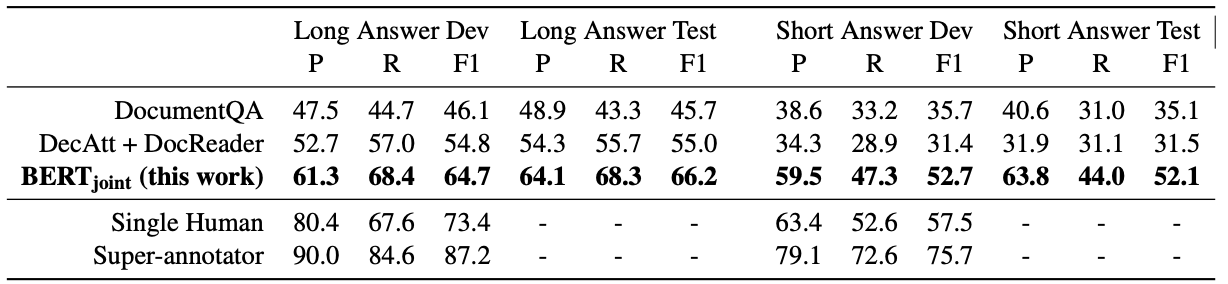
\includegraphics[scale=0.69]{figuras/qa-eda-vshuman.png}
    % \caption[Así aparece el rótulo en el índice]{Así aparece el rótulo en el texto.}
    \caption[Preguntas y Respuestas - Comparación rendimiento BERT vs humanos]{\textbf{En este estudio \cite{BERT_baseline_for_NQ_https://doi.org/10.48550/arxiv.1901.08634} comparan el desempeño de BERT contra un humano común y un humano experto. Se evidencia el mejor desempeño de BERT en ciertos casos. Fuente: \cite{BERT_baseline_for_NQ_https://doi.org/10.48550/arxiv.1901.08634}}}
    \label{fig-qa-eda-vshuman}
\end{figure}

Para evaluar el estado del arte relacionado a la solución de preguntas y respuestas sobre el dataset SQuAD en su versión 1.0 se utilizaron diversas fuentes. 

En el \textit{paper} realizado por \citet{BERT_baseline_for_NQ_https://doi.org/10.48550/arxiv.1901.08634} titulado ``\textit{A BERT Baseline for the Natural Questions}'' los autores concluyen que BERT debe ser la nueva línea base y que constituye un buen punto de partida para los modelos de preguntas y respuestas y \textit{datasets} con características similares. En este mismo estudio los autores comparan el desempeño de BERT con otros modelos que resolvían la tarea en ese momento y además lo compararon con el desempeño de la tarea realizada por un humano común y un humano experto. (ver figura \ref{fig-qa-eda-vshuman}). Los autores concluyen que los resultados obtenidos por los modelos de respuesta a preguntas basados en BERT también se están acercando rápidamente al rendimiento humano informado para estos conjuntos de datos.

Existen otros estudios, como el presentado en el \textit{paper} ``\textit{Comparative Study of Machine Learning Models and BERT on SQuAD}'' de \cite{SQuAD_Comparison_https://doi.org/10.48550/arxiv.2005.11313} donde realizan un análisis comparativo del rendimiento de ciertos modelos populares en el aprendizaje automático y el modelo de BERT sobre SQuAD, brindando BERT una mayor precisión que otros modelos.

En el ranking de la página oficial de SQuAD (\url{https://rajpurkar.github.io/SQuAD-explorer/}) podemos observar muchos modelos basados en ALBERT \cite{ALBERT_https://doi.org/10.48550/arxiv.1909.11942}. ALBERT es una versión de BERT mucho más ligera con 12 millones de parámetros en vez de 110 millones como los que contiene BERT. En el \textit{paper} original de ALBERT llamado ``\textit{ALBERT: A Lite BERT for Self-supervised Learning of Language Representations}''  comparan el desempeño de ALBERT con BERT en las tareas de SQuAD obteniendo resultados bastante similares (ver figura \ref{fig-qa-eda-albert})

\begin{figure}[ht!]
    \centering
    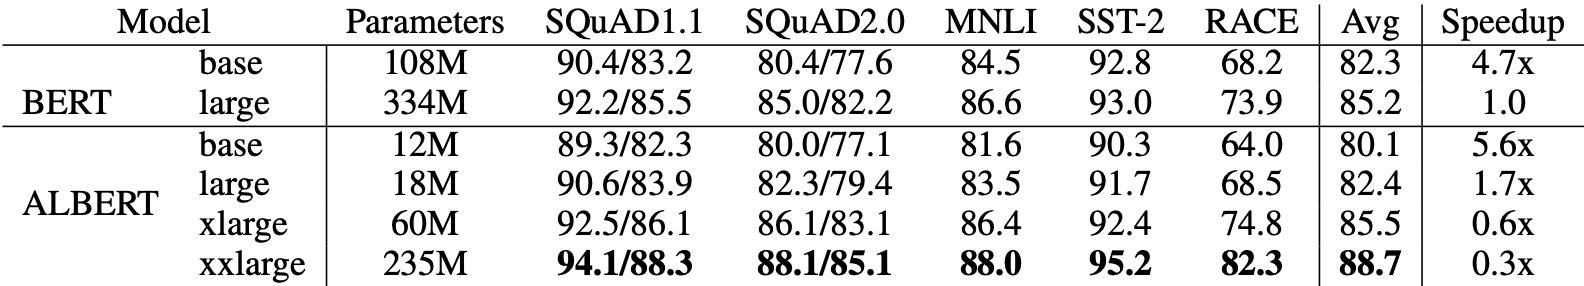
\includegraphics[scale=0.5]{figuras/qa-eda-albert.png}
    % \caption[Así aparece el rótulo en el índice]{Así aparece el rótulo en el texto.}
    \caption[Preguntas y Respuestas - Comparación BERT vs humanos]{\textbf{Comparación de los resultados obtenidos en distintas tareas de NLP entre BERT y su variante ALBERT. Para las tareas SQuAD los dos números equivalen a F1 y EM. Fuente: \cite{ALBERT_https://doi.org/10.48550/arxiv.1909.11942}}}
    \label{fig-qa-eda-albert}
\end{figure}

%%%%%%%%%%%%%%%%%%%%%%%%%%%%%%%%%%%%%%%%%%%%%%%%%%%%%%%%%%%%%%%%%%%%%%%%%%%%%%%%%%%%%%%%%%%%%%%%%%%%%%%%%%%%%%%

\subsection{Arquitectura de la solución}
\label{subsection-qa-arquitectura-de-la-solucion}

Como ya se mencionó en la sección \ref{subsection-arquitectura-bert}, la arquitectura de BERT ha sido diseñada para adaptarse a la resolución de distintos problemas a través de un leve ajuste, por este motivo es que en BERT tenemos dos formas diferentes de manejar la entrada y la salida del modelo. 

Con respecto a la entrada, una de las formas es cuando se tiene un vector que se supone representa toda una frase en su completitud y es básicamente la forma que se utiliza en las tareas de clasificación. La segunda forma de entrada es una lista de vectores, cada uno de los cuales es una representación de las palabras en el contexto que las rodea. Esta segunda forma de entrada es particularmente la que se utiliza en este tipo de problemas al no tratarse de un problema de clasificación como en el experimento anterior.

Como entrada se definieron dos frases, la primera frase representa el texto en el que hay que buscar la información. La segunda frase representa la pregunta que se quiere resolver. En la primera frase, lo que se necesita es buscar dónde empieza y dónde termina la hipotética respuesta a nivel de tokens y ese nivel de tokens luego es traducido a nivel de palabras. De esa forma se busca la respuesta dentro de la primera oración.

Con respecto a la salida, para este caso no se usa el \textit{Pooled Output}, el cual es una representación del token de clasificación [CLS], un embedding de toda la frase. Por el contrario, se usa el \textit{Sequence Output}, el cual está representado por una lista de vectores (embedding), uno para cada una de las palabras, de esta forma se podrá localizar las más probables de ser la el inicio y el final de la respuesta.

Casi siempre que se utiliza BERT para generar la solución de una tarea, lo único que hay que hacer es añadir una capa densa al final antes de hacer ningún ajuste de los parámetros. Estas capas densas se le aplica a cada uno de los elementos, a cada vector y nos va a dar dos posibles respuestas, dos neuronas en la capa de salida.

La primera nos representará una puntuación de qué tan probable es que esa palabra sea la posición inicial en la que empieza la respuesta y la segunda neurona representará una puntuación de qué tan probable es que esa palabra sea la la que finaliza la respuesta De esa forma, simplemente aplicando una capa densa con dos neuronas a cada vector, a cada representación vectorial de las palabras, obtendremos un puntaje de qué tan susceptible es de ser la palabra que inicia o que finaliza la respuesta a la pregunta que estamos buscando.

Finalmente se debe construir un par de listas de todos los puntajes de qué tan probable es que sean el inicio o el final de la respuesta para cada una de las palabras. Una lista para el inicio y otro para el final. La respuesta será la frase o secuencia de palabras contenidas entre el token que tenga el mayor puntaje o probabilidad de ser el inicio de la respuesta y el token con mayor puntaje de ser el final de la respuesta.

Como el proceso de tokenización de BERT tiende a romper palabras, estas se tendrán que reconstruir correctamente.

\begin{figure}[ht!]
    \centering
    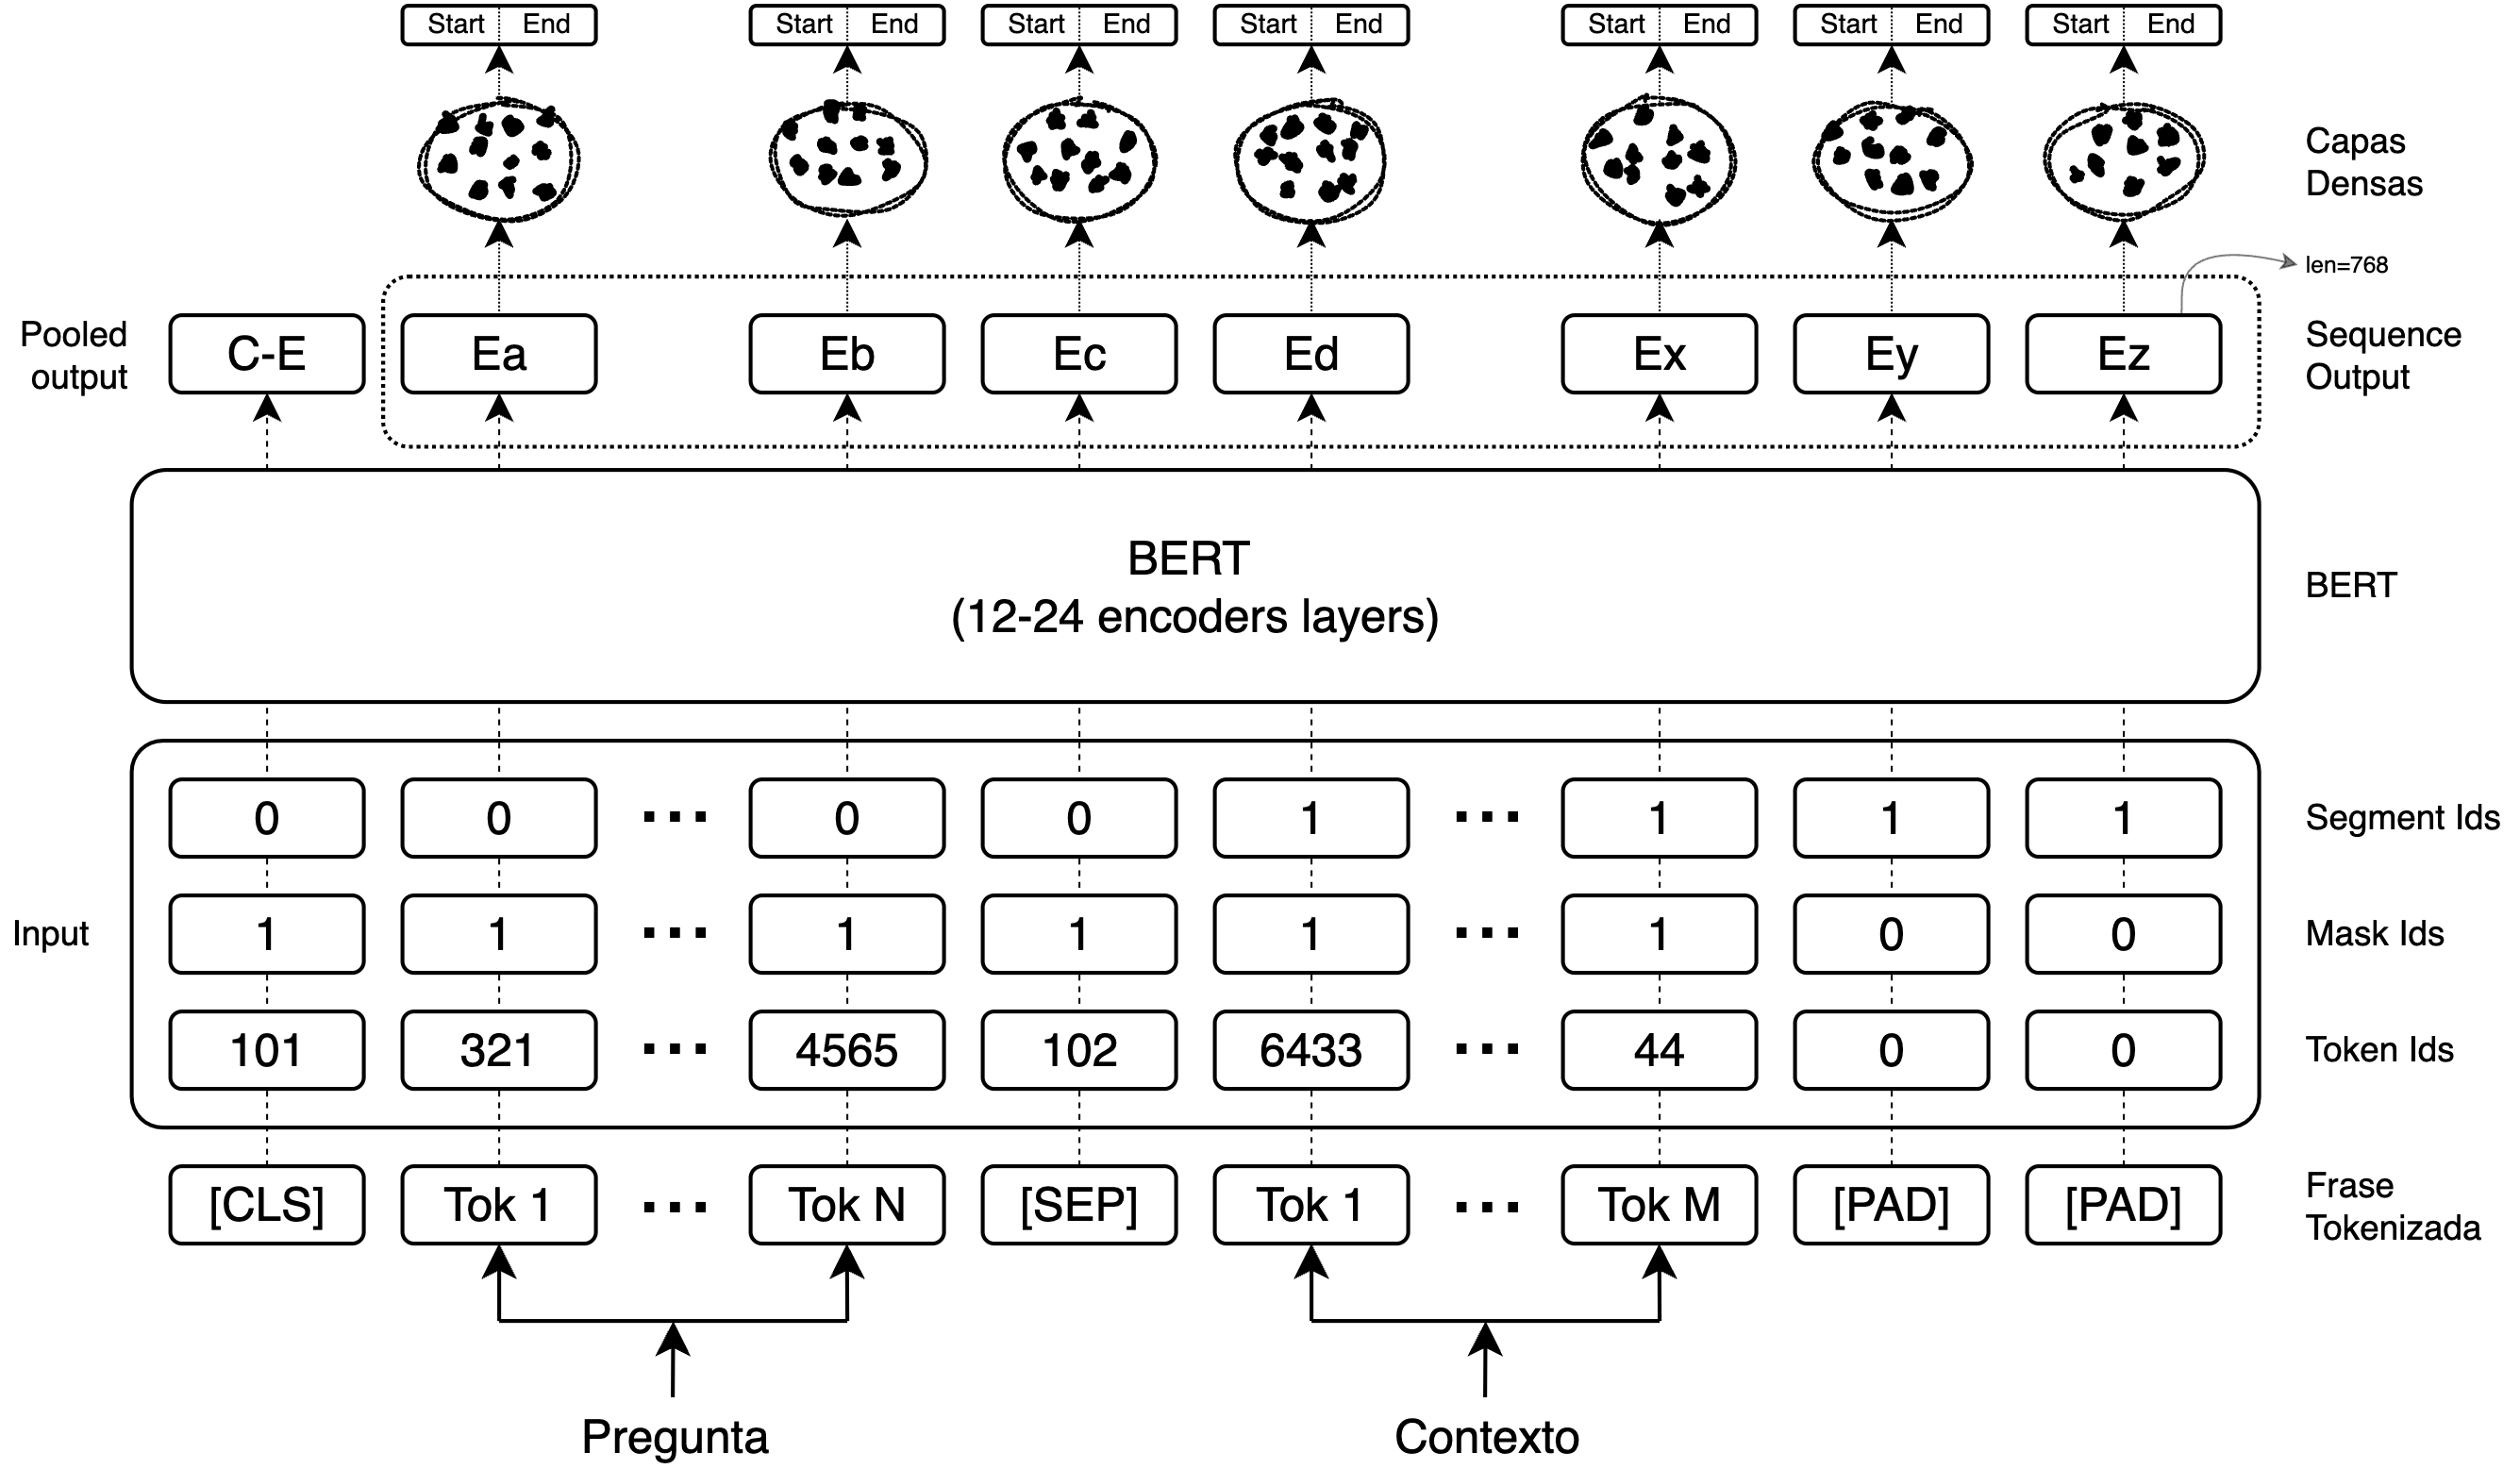
\includegraphics[scale=0.155]{figuras/bert-qa-architecture.png}
    % \caption[Así aparece el rótulo en el índice]{Así aparece el rótulo en el texto.}
    \caption[Preguntas y Respuestas - Arquitectura de la solución]{\textbf{Adecuación de la arquitectura de BERT para la solución de problemas de preguntas y respuestas. Fuente: Imagen propia.}}
    \label{fig-bert-qa-architecture}
\end{figure}

%%%%%%%%%%%%%%%%%%%%%%%%%%%%%%%%%%%%%%%%%%%%%%%%%%%%%%%%%%%%%%%%%%%%%%%%%%%%%%%%%%%%%%%%%%%%%%%%%%%%%%%%%%%%%%%

\subsection{Preparación de los datos}
\label{subsection-qa-preparacion-de-los-datos}

La entrada del modelo BERT para problemas de \textit{question answering} está compuesta por dos frases, la pregunta y el contexto. La forma de manejar la entrada es a través de la estructura mostrada en la figura \ref{fig-bert-qa-architecture}, donde podemos ver:

\begin{enumerate}
    \item Al igual que el experimento anterior y en todos los problemas donde usemos BERT, el token [CLS] se debe anteponer a cada sentencia de entrada. Este token es usado en las tareas de clasificación, pero indistintamente del problema a resolver el modelo BERT siempre espera recibirlo como el comienzo de la entrada.
    \item Seguido al token [CLS] se colocarán los tokens correspondientes a las palabras que componen la pregunta.
    \item A esto le procederá el token especial [SEP] que en este caso tiene un significado distinto dentro de la entrada al experimento anterior. La idea en este caso es que el token [SEP] separará la pregunta del contexto.
    \item En el segment embedding se debe marcar desde el principio de la frase de entrada hasta el token [SEP] como el segmento inicial.
    \item En el resto del token embedding se colocarán los tokens que correspondan al contexto o referencia.
    \item Al igual que en el experimento anterior BERT presenta algunas restricciones con respecto a la entrada:
    \begin{enumerate}
    \item Todas las sentencias de entrada deben tener la misma longitud.
    \item La longitud máxima de la sentencia de entrada es de 384 tokens. Esta longitud es un estándar en el conjunto de datos de SQuAD por dos razones, tener la mayoría de las preguntas y contextos tokenizados sin ningún truncamiento y mantener una longitud limitada para acelerar el entrenamiento.
    \end{enumerate}
\end{enumerate}

A diferencia del problema anterior (ver sección \ref{section-analisis-de-sentimiento}), el conjunto de datos asociado a este problema se encuentra en un \gls{gls_json} que necesita ser preprocesado. Sin embargo, esta tarea de preprocesado de datos es una tarea que se simplifica considerablemente comparado con el proceso del experimento anterior debido a un conjunto de funciones que provee Google para trabajar con el conjunto de datos de SQuAD que ya se encuentran escritas y disponibles en su librería Official.nlp.bert. 

Lo que se logra con estas librerías es transformar los datos de entrenamiento de SQuAD a datos utilizables por las librerías de Tensorflow. Para ello se utilizará la función \textbf{\textit{generate\_tf\_record\_from\_json\_file}}, dejando escrita, su salida, en un
archivo llamado \textbf{\textit{train\_meta\_data}}, divido en cuatro partes. Este archivo ya estará
listo para ser utilizado, también se inicializa el tamaño del batch para el entrenamiento, en este caso será de tamaño 4.

Una vez dado este paso ya se obtienen los datos “tokenizados”, luego a través de la función \textbf{\textit{create\_squad\_dataset}} y a partir de los archivos mencionados con anterioridad, se crea el \textit{dataset} de entrenamiento. De esa forma ya se tendrán listos los datos para entrenar el modelo. 

%%%%%%%%%%%%%%%%%%%%%%%%%%%%%%%%%%%%%%%%%%%%%%%%%%%%%%%%%%%%%%%%%%%%%%%%%%%%%%%%%%%%%%%%%%%%%%%%%%%%%%%%%%%%%%%

\subsection{Modelo y Fine Tuning}
\label{subsection-qa-finetunning}

Al igual que el experimento anterior, el modelo de BERT se obtuvo desde Tensorflow Hub (\url{https://www.tensorflow.org/hub}). Se usó como modelo BERT preentrenado la versión bert\_en\_uncased\_L-12\_H-768\_A-12 al principio se usó la versión bert\_multi\_cased\_L-12\_H-768\_A-12, pensando que se obtendrían mejores resultados usando entradas en distintos idiomas, pero los resultados no fueron buenos. 

Adicionalmente y haciendo uso del API Keras de Tensorflow se creó una ``capa SQuAD'', esta es una capa compuesta por redes neuronales densamente conectadas, la cual será entrenada para devolver dos valores numéricos.

Estos valores representarán dos posiciones en el contexto, que determinarán de dónde se obtendrán el resultado, una vez obtenido el resultado. El resultado calculado se podrá comparar con el resultado esperado y, de esta forma, en base a la evaluación del error cometido, empezar el aprendizaje de las neuronas de la red densamente conectada. 

Como recomienda Tensorflow en su página oficial (\url{https://www.tensorflow.org/text/tutorials/fine_tune_bert}), la función de perdida se implementó a través del método \textbf{\textit{sparse\_categorical\_crossentropy}} de \textbf{\textit{tf.keras.backend}}.

Para entrenar el modelo propuesto se utilizó como valores de los hiperparámetros los recomendados en el \textit{paper} de BERT. Según los autores del \textit{paper} BERT no necesita muchas épocas para ser entrenado y recomiendan que sean entre 2 y 4. \cite{https://doi.org/10.48550/arxiv.1810.04805}:

\begin{itemize}
    \item Tamaño del entrenamiento = 88641 
    \item Número de lotes = 3000 
    \item Tamaño del lote = 4
    \item Tasa de aprendizaje = 2e-5
    \item Longitud máxima de secuencia = 512
    \item Épocas = 3
\end{itemize}

El entrenamiento se realizó usando Google Colab y utilizando la \acrlong{acr_tpu} (\acrshort{acr_tpu}, por sus siglas en inglés). La duración del entrenamiento ha sido:

\begin{itemize}
    \item Primera Época = 12863 segundos.
    \item Segunda Época = 10381 segundos. 
    \item Tercera Época = 11303 segundos.
    \item Entrenamiento total = 34537 segundos, aproximadamente 9 horas y 40 minutos.
\end{itemize}

El código fuente del entrenamiento se encuentra en el repositorio Github \url{https://github.com/lsizaguirre/09MIAR-TFM}

%%%%%%%%%%%%%%%%%%%%%%%%%%%%%%%%%%%%%%%%%%%%%%%%%%%%%%%%%%%%%%%%%%%%%%%%%%%%%%%%%%%%%%%%%%%%%%%%%%%%%%%%%%%%%%%

\subsection{Resultados y Conclusiones.}
\label{subsection-qa-resultados-y-conclusiones}

Este experimento es distinto al anterior en cuanto a la fase de evaluación de los resultados debido a que no se puede hacer de forma directa como en el problema de análisis de sentimiento. 

Para evaluar los modelos, primero se obtienen las predicciones haciendo uso también de un conjunto de funciones que Google pone a disposición para tal fin y estas se usan como entrada para un script de evaluación que se encuentra en la página oficial del \textit{dataset} SQuAD (\url{https://rajpurkar.github.io/SQuAD-explorer/}). 

Este \textit{script} de evaluación en \textit{Python} nos permite evaluar las predicciones bajo las mismas condiciones que son aplicadas en el \textit{paper} de SQuAD (como remover los artículos y signos de puntuación de las frases) y obtener las métricas de Exact Match (EM) y el score F1.

En este caso realizamos dos entrenamientos:

\begin{enumerate}
    \item \textbf{Primer entrenamiento:} \\
    Donde se uso como modelo de BERT la versión bert\_multi\_cased\_L-12\_H-768\_A-12, versión base multilenguaje. Con este modelo obtuvimos las siguientes métricas:
    
    \begin{itemize}
        \item Exact Match (EM) = 29,33\%
        \item F1 Score =  41\%
    \end{itemize}
    
    \item \textbf{Segundo entrenamiento:} \\
    Donde se mantuvieron todos los hiperparámetros con los mismos valores pero se entrenó con va versión bert\_en\_uncased\_L-12\_H-768\_A-12 
    
    \begin{itemize}
        \item Exact Match (EM) = 71,34\%
        \item F1 Score =  80,58\%
    \end{itemize}
    
\end{enumerate}

Con respecto a los resultados podemos deducir:

\begin{itemize}
    \item En el primer entrenamiento no se obtuvieron buenos resultados debido a que no seleccionamos el mejor modelo de BERT con respecto a los datos de entrenamiento. Se eligió trabajar con un modelo multilenguaje cuando en los datos de entrenamiento hay solo frases en ingles, además usamos un modelo entrenado con minúsculas y mayúsculas cuando el script de evaluación transforma cada frase a minúscula en el proceso de evaluación.
    \item En el segundo entrenamiento haciendo uso de un modelo adecuado los resultados fueron bastantes satisfactorios, acercándose a los estándares que definen el estado del arte y muy similares a las capacidades humanas.
\end{itemize}